% !TEX encoding = UTF-8
% !TEX TS-program = pdflatex
% !TEX root = ../tesi.tex

%**************************************************************
\chapter{Analisi dei requisiti}
\label{cap:analisi-requisiti}
%**************************************************************

\intro{Breve introduzione al capitolo}\\
Questo capitolo ha lo scopo di fornire una definizione dei requisiti individuati per la creazione del prodotto Identity Wallet (IW). Le metodologie usate sono tratte dal capitolo quattro di \cite{som:swe}.
Più in particolare il presente capitolo si prefigge di: 
\begin{itemize}
    \item individuare le fonti per la deduzione dei requisiti; 
    \item dedurre i requisiti dalle fonti; 
    \item descrivere i requisiti individuati; 
    \item catalogare i requisiti individuati; 
    \item fissare un ordine di priorità tra i requisiti individuati;
\end{itemize}
\section{Specifiche in Linguaggio Naturale}
Il linguaggio naturale ha un’enorme potenza espressiva ma essendo inerentemente ambiguo può portare ad incomprensioni; è quindi necessario limitarne l’utilizzo e standardizzarlo, in modo da ridurre al minimo le possibili ambiguità. È comunque fondamentale evitare di utilizzare espressioni e acronimi che possano essere fraintendibili dagli stakeholders, a tal proposito in fondo al documento è presente una lista degli acronimi utilizzati.
\section{Specifiche in Linguaggio Strutturato}
Il linguaggio strutturato mantiene gran parte dell’espressività del linguaggio naturale, fornendo però uno standard schematico che permette l’uniformità della descrizione dei vari requisiti. Sebbene l’utilizzo di un linguaggio strutturato permetta di organizzare i requisiti in modo più ordinato e comprensibile, talvolta la ridotta espressività rende difficile la definizione di requisiti complessi. A tal proposito è possibile integrare la specifica in linguaggio strutturato con una descrizione in linguaggio naturale.
\section{Specifiche in Linguaggio UML Use Case}
Per la definizione dei diagrammi UML dei casi d’uso, viene utilizzato lo standard UML 2.0 \footcite{site:uml}. Nei diagrammi dei casi d’uso vengono mostrati gli attori coinvolti in un’interazione con il sistema in modo schematico, indicando i nomi delle parti coinvolte. Eventuali informazioni aggiuntive possono essere espresse testualmente.

\section{Analisi dei requisiti IW}
\subsection{Casi d'uso}

Per lo studio dei casi di utilizzo del prodotto sono stati creati dei diagrammi.
I diagrammi dei casi d'uso (in inglese \emph{Use Case Diagram}) sono diagrammi di tipo \gls{uml} dedicati alla descrizione delle funzioni o dei servizi offerti da un sistema, così come sono percepiti e utilizzati dagli attori che interagiscono col sistema stesso.

\subsubsection{Descrizione Attori}
I tipi di attori principali che andranno ad interagire direttamente con il sistema sono essenzialmente tre: 
\begin{itemize}
    \item utente;
    \item utente non registrato;
    \item utente autenticato. 
\end{itemize}   
Tra di essi è presente una relazione di generalizzazione che vede l’attore utente come generalizzazione degli attori utente non registrato e utente registrato. Questo tipo di generalizzazione viene rappresentata graficamente in figura \ref{fig:ger-actors}.
\begin{figure}[!h]
    
    \centering
    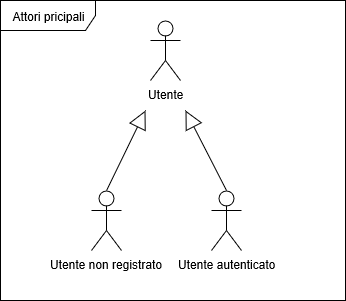
\includegraphics[width=0.5\columnwidth]{usecase/use-case-iw/actors.png} 
    \caption{Gerarchia utenti user case}
    \label{fig:ger-actors} 
\end{figure}
Sono stati individuati i seguenti attori secondari: ITF, \textit{MonoKee}.
\paragraph{Attori principali}
\begin{itemize}
    \item \textbf{Utente}: l’attore utente è un fruitore generico del sistema. Potrebbe avere o non avere effettuato l’accesso all’applicazione. Da lui derivano gli attori utente non registrato e utente autenticato.	
    \item \textbf{Utente non registrato}: l’attore utente non registrato è una particolare specializzazione dell’attore utente. Unica sua caratteristica è quella di non essere riconosciuto come utente di \textit{MonoKee}.
    \item \textbf{Utente autenticato}: l’attore utente autenticato è una particolare specializzazione dell’attore utente. Rappresenta un utente che ha effettuato l’accesso al sistema e che è stato riconosciuto all’interno del sistema \textit{MonoKee}.
\end{itemize}
      
\paragraph{Attori secondari}
\begin{itemize}
    \item \textbf{ITF}: è il componente dell’estensione che ha il compito di conservare e convalidare tutte le informazioni provenienti dall’IW.
    \item \textbf{MonoKee}: è il componente centrare dell’attuale servizio \textit{MonoKee}. Ha il compito di fornire le informazioni di accesso del servizio \textit{MonoKee}. 
\end{itemize}
    


\subsubsection{UC1: Azioni utente generico}
\begin{figure}[!htbp] 
    \centering 
    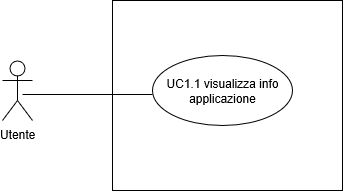
\includegraphics[width=0.7\columnwidth]{usecase/use-case-iw/UC1-azioni-utente.png} 
    \caption{Use Case - UC1: Azioni utente generico}
\end{figure}

\paragraph{Descrizione}  L’utente può visualizzare le informazioni sull’applicazione 
\paragraph{Attore primario}  Utente
\paragraph{Attore secondario}  Nessuno
\paragraph{Precondizioni}  L’utente ha avviato l’applicazione
\paragraph{Postcondizioni}  L’utente ha eseguito le azioni che desiderava compiere in relazione alle sue possibilità
\paragraph{Scenario principale}  
    \begin{enumerate}
        \item UC1.1 Visualizza info applicazione
    \end{enumerate}
\paragraph{Scenari alternativi}  Nessuno


\subsubsection{UC1.1 – Visualizza info applicazione}
\begin{figure}[!htbp] 
    \centering 
    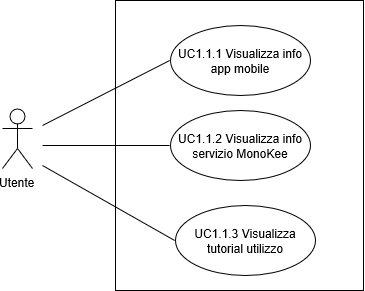
\includegraphics[width=0.7\columnwidth]{usecase/use-case-iw/UC1-1-Visualizza-info-applicazione.png} 
    \caption{Use Case - UC1.1 – Visualizza info applicazione}
\end{figure}

\paragraph{Descrizione}  Il sistema deve visualizzare le informazioni relative all’applicazione mobile e al servizio MonoKee  
\paragraph{Attore primario}  Utente
\paragraph{Attore secondario}  Nessuno
\paragraph{Precondizioni}  L’utente ha avviato l’applicazione
\paragraph{Postcondizioni}  L’utente ha visualizzato le informazioni che desirava riguardo l’applicazione
\paragraph{Scenario principale}  
    \begin{enumerate}
        \item UC1.1.1 Visualizza info applicazione
        \item UC1.1.2 Visualizza info servizio MonoKee
        \item UC1.1.3 Visualizza tutorial utilizzo
    \end{enumerate}
\paragraph{Scenari alternativi}  Nessuno


\subsubsection{UC1.1.1 – Visualizza info app mobile}
\paragraph{Descrizione}  Il sistema deve visualizzare le informazioni tecniche relative all’applicazione mobile
\paragraph{Attore primario}  Utente
\paragraph{Attore secondario}  Nessuno
\paragraph{Precondizioni}  L’utente ha avviato l’applicazione ed ha richiesto la visualizzazione delle informazioni tecniche relative all’applicazione mobile
\paragraph{Postcondizioni}  L’utente ha visualizzato le informazioni con le informazioni tecniche relative all’applicazione mobile
\paragraph{Scenario principale}  
L’utente visualizza un messaggio con le informazioni tecniche relative all’applicazione mobile
\paragraph{Scenari alternativi}  Nessuno


\subsubsection{UC1.1.2 – Visualizza info servizio MonoKee}
\paragraph{Descrizione}  Il sistema deve visualizzare le informazioni relative al servizio \textit{MonoKee}
\paragraph{Attore primario}  Utente
\paragraph{Attore secondario}  Nessuno
\paragraph{Precondizioni}  L’utente ha avviato l’applicazione ed ha richiesto la visualizzazione delle informazioni relative al servizio \textit{MonoKee}
\paragraph{Postcondizioni}  L’utente ha visualizzato le informazioni con le informazioni relative al servizio \textit{MonoKee}
\paragraph{Scenario principale}  
L’utente visualizza un messaggio con le informazioni relative al servizio MonoKee
\paragraph{Scenari alternativi}  Nessuno


\subsubsection{UC1.1.3 – Visualizza tutorial utilizzo}
\paragraph{Descrizione}  Il sistema deve visualizzare un tutorial su come utilizzare l’applicazione IW
\paragraph{Attore primario}  Utente
\paragraph{Attore secondario}  Nessuno
\paragraph{Precondizioni}  L’utente ha avviato l’applicazione ed ha richiesto la visualizzazione di un tutorial su come utilizzare l’applicazione IW
\paragraph{Postcondizioni}  L’utente ha visualizzato il tutorial su come utilizzare l’applicazione IW
\paragraph{Scenario principale}  
L’utente visualizza un tutorial su come utilizzare l’applicazione IW
\paragraph{Scenari alternativi}  Nessuno


\subsubsection{UC2 – Azioni utente non registrato}
\begin{figure}[!htbp] 
    \centering 
    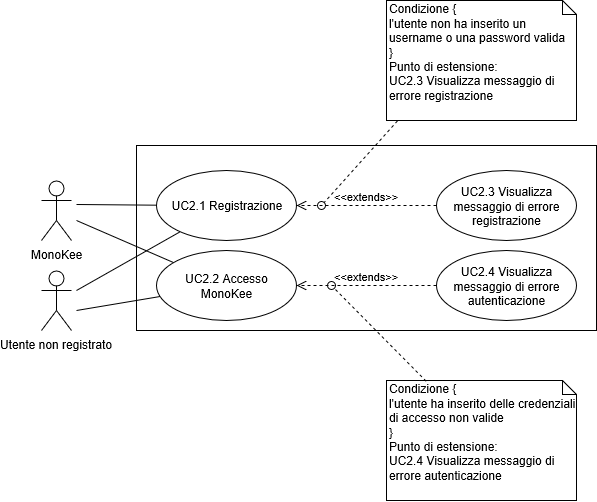
\includegraphics[width=0.7\columnwidth]{usecase/use-case-iw/UC2-azioni-utente-non-registrato.png} 
    \caption{Use Case - UC2: Azioni utente non registrato}
\end{figure}

\paragraph{Descrizione}  L’utente non registrato può eseguire le operazioni di registrazione e accesso al servizio \textit{MonoKee} 
\paragraph{Attore primario}  Utente non registrato
\paragraph{Attore secondario}  \textit{MonoKee}
\paragraph{Precondizioni}  L’utente ha avviato l’applicazione ed non è ancora riconosciuto nel sistema
\paragraph{Postcondizioni}  L’utente ha eseguito le azioni che desiderava compiere in relazione alla condizione di non essere registrato
\paragraph{Scenario principale}  
    \begin{enumerate}
        \item UC2.1 Registrazione
        \item UC2.2 Accesso \textit{MonoKee}
    \end{enumerate}
\paragraph{Scenari alternativi}  
    \begin{enumerate}
        \item l’utente ha fornito dati di registrazione non validi o il doppio inserimento della password non coincide: UC2.3 Visualizzazione messaggio di errore registrazione.
        \item l’utente ha fornito username e password non corrispondenti ha nessun utente registrato al servizio: UC2.4 Visualizzazione messaggio di errore autenticazione.
    \end{enumerate}


\subsubsection{UC2.1 – Registrazione}
\begin{figure}[!htbp] 
    \centering 
    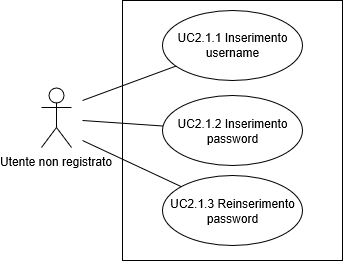
\includegraphics[width=0.7\columnwidth]{usecase/use-case-iw/UC2-1-Registrazione.png} 
    \caption{Use Case - UC2.1: Registrazione}
\end{figure}

\paragraph{Descrizione}  L’utente non registrato può eseguire l’operazione di registrazione 
\paragraph{Attore primario}  Utente non registrato
\paragraph{Attore secondario}  \textit{MonoKee}
\paragraph{Precondizioni}  L’utente ha avviato l’applicazione, non è ancora riconosciuto nel sistema ed ha espresso la volontà di effettuare la registrazione al servizio \textit{MonoKee}
\paragraph{Postcondizioni}  L’utente ha eseguito l’operazione di registrazione al sistema
\paragraph{Scenario principale}  
    \begin{enumerate}
        \item UC2.1.1 Inserimento username
        \item UC2.1.2 Inserimento password
        \item UC2.1.3 Reinserimento password
    \end{enumerate}
\paragraph{Scenari alternativi}  Nessuno



\subsubsection{UC2.1.1 – Inserimento username}
\paragraph{Descrizione}  L’utente non registrato deve inserire un username per l’operazione di registrazione
\paragraph{Attore primario}  Utente non registrato
\paragraph{Attore secondario}  Nessuno
\paragraph{Precondizioni}  L’utente ha avviato l’applicazione, non è ancora riconosciuto nel sistema ed il sistema richiede l’inserimento di un username per l’operazione di registrazione
\paragraph{Postcondizioni}  L’utente ha inserito l’username per la registrazione
\paragraph{Scenario principale}  
L’utente non registrato inserisce una stringa tramite l’utilizzo di una \textit{text box}
\paragraph{Scenari alternativi}  Nessuno


\subsubsection{UC2.1.2 – Inserimento password}
\paragraph{Descrizione}  L’utente non registrato deve inserire una password per l’operazione di registrazione
\paragraph{Attore primario}  Utente non registrato
\paragraph{Attore secondario}  Nessuno
\paragraph{Precondizioni}  L’utente ha avviato l’applicazione, non è ancora riconosciuto nel sistema ed il sistema richiede l’inserimento di una password per l’operazione di registrazione
\paragraph{Postcondizioni}  L’utente ha inserito la password per la registrazione
\paragraph{Scenario principale}  
L’utente non registrato inserisce una stringa tramite l’utilizzo di una \textit{text box}
\paragraph{Scenari alternativi}  Nessuno



\subsubsection{UC2.1.3 – Reinserimento password}
\paragraph{Descrizione}  L’utente non registrato deve reinserire la password per l’operazione di registrazione
\paragraph{Attore primario}  Utente non registrato
\paragraph{Attore secondario}  Nessuno
\paragraph{Precondizioni}  L’utente ha avviato l’applicazione, non è ancora riconosciuto nel sistema ed il sistema richiede il reinserimento di una password per l’operazione di registrazione
\paragraph{Postcondizioni}  L’utente ha reinserito la password per la registrazione
\paragraph{Scenario principale}  
L’utente non registrato inserisce una stringa tramite l’utilizzo di una \textit{text box}
\paragraph{Scenari alternativi}  Nessuno



\subsubsection{UC2.2 – Accesso MonoKee}
\begin{figure}[!htbp] 
    \centering 
    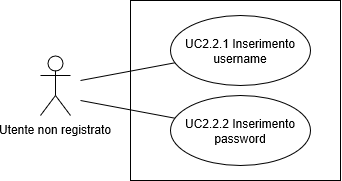
\includegraphics[width=0.7\columnwidth]{usecase/use-case-iw/UC2-2-Accesso-MonoKee.png} 
    \caption{Use Case - UC2.1: Accesso MonoKee}
\end{figure}

\paragraph{Descrizione}  L’utente non registrato può eseguire l’operazione di autenticazione 
\paragraph{Attore primario}  Utente non registrato
\paragraph{Attore secondario}  \textit{MonoKee}
\paragraph{Precondizioni}  L’utente ha avviato l’applicazione, non è ancora riconosciuto nel sistema ed ha espresso la volontà di effettuare l’autenticazione al servizio \textit{MonoKee}
\paragraph{Postcondizioni}  L’utente ha eseguito l’operazione di accesso al sistema ed è quindi ora riconosciuto come utente autenticato
\paragraph{Scenario principale}  
    \begin{enumerate}
        \item UC2.1.1 Inserimento username
        \item UC2.1.2 Inserimento password
    \end{enumerate}
\paragraph{Scenari alternativi}  Nessuno


\subsubsection{UC2.2.1 – Inserimento username}
\paragraph{Descrizione}  L’utente non registrato deve inserire un \textit{username} per l’operazione di autenticazione
\paragraph{Attore primario}  Utente non registrato
\paragraph{Attore secondario}  Nessuno
\paragraph{Precondizioni}  L’utente ha avviato l’applicazione, non è ancora riconosciuto nel sistema ed il sistema richiede l’inserimento di un \textit{username} per l’operazione di autenticazione
\paragraph{Postcondizioni}  L’utente ha inserito \textit{username} per l’autenticazione
\paragraph{Scenario principale}  
L’utente non registrato inserisce una stringa tramite l’utilizzo di una \textit{text box}
\paragraph{Scenari alternativi}  Nessuno



\subsubsection{UC2.2.2 – Inserimento password}
\paragraph{Descrizione}  L’utente non registrato deve inserire una password per l’operazione di autenticazione
\paragraph{Attore primario}  Utente non registrato
\paragraph{Attore secondario}  Nessuno
\paragraph{Precondizioni}  L’utente ha avviato l’applicazione, non è ancora riconosciuto nel sistema ed il sistema richiede l’inserimento di una password per l’operazione di autentificazione
\paragraph{Postcondizioni}  L’utente ha inserito la password per l’autentificazione
\paragraph{Scenario principale}  
L’utente non registrato inserisce una stringa tramite l’utilizzo di una \textit{text box}
\paragraph{Scenari alternativi}  Nessuno



\subsubsection{UC2.3 – Visualizza messaggio di errore registrazione}
\paragraph{Descrizione}  L’utente non registrato fornisce username già esistente o il doppio inserimento della password non coincide
\paragraph{Attore primario}  Utente non registrato
\paragraph{Attore secondario}  Nessuno
\paragraph{Precondizioni}  L’utente ha avviato l’applicazione, non è ancora riconosciuto nel sistema ed il sistema ha inserito un \textit{username} già esistente o delle password non coincidenti durante la registrazionerichiede l’inserimento di una password per l’operazione di autentificazione
\paragraph{Postcondizioni}  L’utente ha visualizzato un messaggio di errore relativo all’impossibilità di effettuare la registrazione con i dati forniti
\paragraph{Scenario principale}  
L’utente visualizza un messaggio di errore relativo all’impossibilità di effettuare la registrazione con i dati forniti
\paragraph{Scenari alternativi}  Nessuno



\subsubsection{UC2.4 – Visualizza messaggio di errore autenticazione}
\paragraph{Descrizione}  L’utente non registrato fornisce username e password che non corrispondono a nessun utente registrato al servizio \textit{MonoKee}
\paragraph{Attore primario}  Utente non registrato
\paragraph{Attore secondario}  Nessuno
\paragraph{Precondizioni}  L’utente ha avviato l’applicazione, non è ancora riconosciuto nel sistema ed il sistema ha inserito un username e una password che non corrispondono a nessun utente registrato al servizio \textit{MonoKee}
\paragraph{Postcondizioni}  L’utente ha visualizzato un messaggio di errore relativo all’impossibilità di effettuare l’autenticazione
\paragraph{Scenario principale}  
L’utente visualizza un messaggio di errore relativo all’impossibilità di effettuare l’autenticazione
\paragraph{Scenari alternativi}  Nessuno



\subsubsection{UC3 – Azioni utente autenticato}
\begin{figure}[!htbp] 
    \centering 
    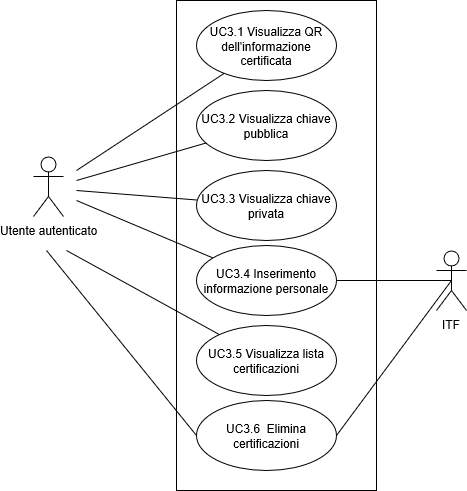
\includegraphics[width=0.7\columnwidth]{usecase/use-case-iw/UC3-Azioni-utente-autententicato.png} 
    \caption{Use Case - UC3: Azioni utente autenticato}
\end{figure}

\paragraph{Descrizione}  L’utente autenticato può eseguire le operazioni legate alla gestione della sua identità e alla presentazione dei propri dati ad un SP
\paragraph{Attore primario}  Utente Autenticato
\paragraph{Attore secondario}  ITF
\paragraph{Precondizioni}  L’utente ha avviato l’applicazione ed è riconosciuto nel sistema come utente di \textit{MonoKee}
\paragraph{Postcondizioni}  L’utente ha eseguito le azioni che desiderava compiere in relazione alla condizione essere riconosciuto come utente di \textit{MonoKee}
\paragraph{Scenario principale}  
    \begin{enumerate}
        \item UC3.1 Visualizza QR dell’informazione certificata
        \item UC3.2 Visualizza chiave pubblica
        \item UC3.3 Visualizza chiave privata
        \item UC3.4 Inserimento informazione personale
        \item UC3.5 Visualizza lista certificazioni
        \item UC3.6 Elimina certificazione
    \end{enumerate}
\paragraph{Scenari alternativi}  Nessuno





\subsubsection{UC3.1 – Visualizza QR dell’informazione certificata}
\paragraph{Descrizione}  L’utente autenticato può visualizzare nel proprio schermo un codice QR che rappresenta un’informazione certificata
\paragraph{Attore primario}  Utente Autenticato
\paragraph{Attore secondario}  Nessuno
\paragraph{Precondizioni}  L’utente ha avviato l’applicazione, è riconosciuto nel sistema come utente di \textit{MonoKee} e ha richiesto di visualizzare il codice QR di una certificazione precedentemente inserita.
\paragraph{Postcondizioni}  L’utente ha visualizzato il codice QR che rappresenta la certificazione selezionata
\paragraph{Scenario principale}  
L’utente seleziona e poi visualizza il codice QR che rappresenta la certificazione selezionata
\paragraph{Scenari alternativi}  Nessuno


\subsubsection{UC3.2 – Visualizza chiave pubblica}
\paragraph{Descrizione}  L’utente autenticato può visualizzare la chiave pubblica generata al momento della registrazione
\paragraph{Attore primario}  Utente Autenticato
\paragraph{Attore secondario}  Nessuno
\paragraph{Precondizioni}  L’utente ha avviato l’applicazione, è riconosciuto nel sistema come utente di \textit{MonoKee} e ha richiesto la visualizzazione della chiave pubblica.
\paragraph{Postcondizioni}  L’utente ha visualizzato la propria chiave pubblica precedentemente generata
\paragraph{Scenario principale}  
L’utente visualizza la propria chiave pubblica precedentemente generata
\paragraph{Scenari alternativi}  Nessuno



\subsubsection{UC3.2 – Visualizza chiave privata}
\paragraph{Descrizione}  L’utente autenticato può visualizzare la chiave privata generata al momento della registrazione
\paragraph{Attore primario}  Utente Autenticato
\paragraph{Attore secondario}  Nessuno
\paragraph{Precondizioni}  L’utente ha avviato l’applicazione, è riconosciuto nel sistema come utente di \textit{MonoKee} e ha richiesto la visualizzazione della chiave privata.
\paragraph{Postcondizioni}  L’utente ha visualizzato la propria chiave privata precedentemente generata
\paragraph{Scenario principale}  
L’utente visualizza la propria chiave privata precedentemente generata
\paragraph{Scenari alternativi}  Nessuno



\subsubsection{UC3.4 – Inserimento informazione personale}
\begin{figure}[!htbp] 
    \centering 
    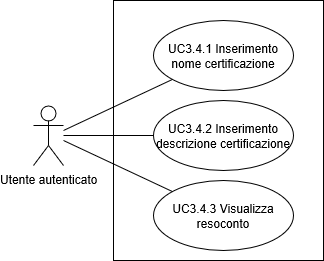
\includegraphics[width=0.7\columnwidth]{usecase/use-case-iw/UC3-4-Inserimento-informazione-personale.png} 
    \caption{Use Case - UC3.4: Inserimento informazione personale}
\end{figure}

\paragraph{Descrizione}  L’utente autenticato può inserire una certificazione e sottometterla all’ITF
\paragraph{Attore primario}  Utente Autenticato
\paragraph{Attore secondario}  ITF
\paragraph{Precondizioni}  L’utente ha avviato l’applicazione, è riconosciuto nel sistema come utente di \textit{MonoKee}, e ha intende inserire una nuova certificazione alla propria identità
\paragraph{Postcondizioni}  L’utente ha inserito la certificazione e questa è stata presentata all’ITF
\paragraph{Scenario principale}  
    \begin{enumerate}
        \item UC3.4.1 Inserimento nome certificazione
        \item UC3.4.2 Inserimento descrizione certificazione
        \item UC3.4.3 Visualizza resoconto
    \end{enumerate}
\paragraph{Scenari alternativi}  Nessuno



\subsubsection{UC3.4.1 – Inserimento nome certificazione}
\paragraph{Descrizione}  L’utente autenticato deve inserire un nome per l’operazione di inserimento certificazione
\paragraph{Attore primario}  Utente Autenticato
\paragraph{Attore secondario}  Nessuno
\paragraph{Precondizioni}  L’utente ha avviato l’applicazione, è riconosciuto nel sistema ed il sistema richiede l’inserimento di un nome per l’operazione di inserimento certificazione
\paragraph{Postcondizioni}  L’utente ha inserito il nome per l’inserimento della certificazione
\paragraph{Scenario principale}  
L’utente autenticato inserisce una stringa tramite l’utilizzo di una \textit{text box}
\paragraph{Scenari alternativi}  Nessuno



\subsubsection{UC3.4.2 – Inserimento descrizione certificazione}
\paragraph{Descrizione}  L’utente autenticato deve inserire una descrizione per l’operazione di inserimento certificazione
\paragraph{Attore primario}  Utente Autenticato
\paragraph{Attore secondario}  Nessuno
\paragraph{Precondizioni} L’utente ha avviato l’applicazione, è riconosciuto nel sistema ed il sistema richiede l’inserimento di una descrizione per l’operazione di inserimento certificazione
\paragraph{Postcondizioni}  L’utente ha inserito la descrizione per l’inserimento della certificazione
\paragraph{Scenario principale}  
L’utente autenticato inserisce un insieme di stringhe tramite l’utilizzo di una \textit{text box}
\paragraph{Scenari alternativi}  Nessuno




\subsubsection{UC3.4.3 – Visualizza resoconto}
\paragraph{Descrizione}  L’utente autenticato può visualizzare un resoconto dei dati inseriti durante la procedura di inserimento certificazione
\paragraph{Attore primario}  Utente Autenticato
\paragraph{Attore secondario}  Nessuno
\paragraph{Precondizioni} L’utente ha avviato l’applicazione, è riconosciuto nel sistema come utente di \textit{MonoKee}, ha iniziato una procedura di inserimento certificazione e ha richiesto la visualizzazione del resoconto dei dati inseriti
\paragraph{Postcondizioni}  L’utente ha visualizzato un resoconto dei dati inseriti durante la procedura di inserimento certificazione
\paragraph{Scenario principale}  
L’utente visualizza un resoconto dei dati inseriti durante la procedura di inserimento certificazione
\paragraph{Scenari alternativi}  Nessuno






\subsubsection{UC3.5 – Visualizza lista certificazioni}
\begin{figure}[!htbp] 
    \centering 
    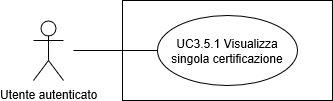
\includegraphics[width=0.7\columnwidth]{usecase/use-case-iw/UC3-5-Visualizza-lista-certificazioni.png} 
    \caption{Use Case - UC3.5: Visualizza lista certificazioni}
\end{figure}

\paragraph{Descrizione}  L’utente autenticato può visualizzare una lista con il nome e l’identificativo della certificazione associate alla propria identità
\paragraph{Attore primario}  Utente Autenticato
\paragraph{Attore secondario}  Nessuno
\paragraph{Precondizioni}  L’utente ha avviato l’applicazione, è riconosciuto nel sistema come utente di MonoKee e ha richiesto la visualizzazione della lista delle certificazioni
\paragraph{Postcondizioni}  L’utente ha visualizzato la lista delle certificazioni
\paragraph{Scenario principale}  
    \begin{enumerate}
        \item UC3.5.1 Visualizza singola certificazione
    \end{enumerate}
\paragraph{Scenari alternativi}  Nessuno





\subsubsection{UC3.5.1 – Visualizza singola certificazione}
\begin{figure}[!htbp] 
    \centering 
    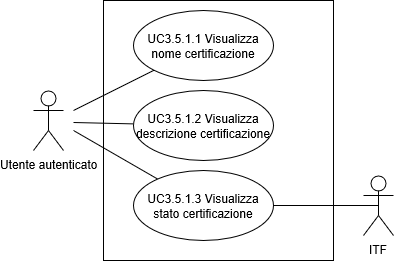
\includegraphics[width=0.7\columnwidth]{usecase/use-case-iw/UC3-5-1-Visualizza-singola-certificazione.png} 
    \caption{Use Case - UC3.5.1: Visualizza singola certificazione}
\end{figure}

\paragraph{Descrizione}  L’utente autenticato può visualizzare i dettagli di una certificazione selezionata della lista delle certificazioni
\paragraph{Attore primario}  Utente Autenticato
\paragraph{Attore secondario}  ITF
\paragraph{Precondizioni}  L’utente ha avviato l’applicazione, è riconosciuto nel sistema come utente di \textit{MonoKee} e ha richiesto la visualizzazione di una specifica \textit{entry} della lista delle certificazioni
\paragraph{Postcondizioni}  L’utente ha visualizzato i dettagli di una specifica certificazione della lista
\paragraph{Scenario principale}  
    \begin{enumerate}
        \item UC3.5.1.1 Visualizza nome certificazione
        \item UC3.5.1.2 Visualizza descrizione certificazione
        \item UC3.5.1.3 Visualizza stato certificazione
    \end{enumerate}
\paragraph{Scenari alternativi}  Nessuno




\subsubsection{UC3.5.1.1 – Visualizza nome certificazione}
\paragraph{Descrizione}  L’utente autenticato può visualizzare il nome di una certificazione selezionata della lista delle certificazioni
\paragraph{Attore primario}  Utente Autenticato
\paragraph{Attore secondario}  Nessuno
\paragraph{Precondizioni} L’utente ha avviato l’applicazione, è riconosciuto nel sistema come utente di \textit{MonoKee} e ha richiesto la visualizzazione del nome di una specifica \textit{entry} della lista delle certificazioni
\paragraph{Postcondizioni}  L’utente ha visualizzato il nome di una specifica certificazione della lista
\paragraph{Scenario principale}  
L’utente visualizza il nome di una specifica certificazione della lista
\paragraph{Scenari alternativi}  Nessuno




\subsubsection{UC3.5.1.2 – Visualizza descrizione certificazione}
\paragraph{Descrizione}  L’utente autenticato può visualizzare la descrizione di una certificazione selezionata della lista delle certificazioni
\paragraph{Attore primario}  Utente Autenticato
\paragraph{Attore secondario}  Nessuno
\paragraph{Precondizioni} L’utente ha avviato l’applicazione, è riconosciuto nel sistema come utente di \textit{MonoKee} e ha richiesto la visualizzazione della descrizione di una specifica \textit{entry} della lista delle certificazioni
\paragraph{Postcondizioni}  L’utente ha visualizzato la descrizione di una specifica certificazione della lista
\paragraph{Scenario principale}  
L’utente visualizza la descrizione di una specifica certificazione della lista
\paragraph{Scenari alternativi}  Nessuno



\subsubsection{UC3.5.1.3 – Visualizza stato certificazione}
\paragraph{Descrizione}  L’utente autenticato può visualizzare lo stato di una certificazione selezionata della lista delle certificazioni. L’informazione proviene dall’ITF.
\paragraph{Attore primario}  Utente Autenticato
\paragraph{Attore secondario}  ITF
\paragraph{Precondizioni} L’utente ha avviato l’applicazione, è riconosciuto nel sistema come utente di \textit{MonoKee} e ha richiesto la visualizzazione dello stato di una specifica \textit{entry} della lista delle certificazioni
\paragraph{Postcondizioni}  L’utente ha visualizzato lo stato di una specifica certificazione della lista
\paragraph{Scenario principale}  
L’utente visualizza una stringa che può essere confermata da un TTP o non confermata.
\paragraph{Scenari alternativi}  Nessuno



\subsubsection{UC3.6 – Elimina certificazione}
\paragraph{Descrizione}  L’utente autenticato può eliminare una certificazione selezionata
\paragraph{Attore primario}  Utente Autenticato
\paragraph{Attore secondario}  ITF
\paragraph{Precondizioni} L’utente ha avviato l’applicazione, è riconosciuto nel sistema come utente di MonoKee e ha richiesto l’eliminazione di una specifica certificazione
\paragraph{Postcondizioni}  La certificazione non è più presente dal sistema e pure dall’ITF
\paragraph{Scenario principale}  
L’utente seleziona e poi esprime la volontà di eliminare la certificazione certificata
\paragraph{Scenari alternativi}  Nessuno

















\newpage
\subsection{Tracciamento dei requisiti}

\subsubsection{Fonti}
Per la deduzione dei requisiti utente e di sistema, che verranno presentati nelle sezioni a seguire, sono stati usati come fonti lo studio \textit{Gartner} \footcite{farah:The-Dawn-of-Decentralized-Identity}, il capitolo \emph{Studio di fattibilità IW} e gli \textit{Use Case} presentati nella sezione \emph{Casi d'uso}. La struttura e le convenzioni usate sono ispirate dal capitolo di \cite{som:swe}. In seguito vengono riportate le categorie che vengono usate per la catalogazione:
\begin{itemize}
    \item F: requisito funzionale;
    \item V: requisito di vincolo;
    \item Q: requisito di qualità.
\end{itemize}
    
Per l’attribuzione della priorità viene usata la tecnica \textit{MoSCoW}, quindi gli indici usati sono i seguenti:
\begin{itemize}
    \item M: must;
    \item S: should; 
    \item C: could; 
    \item W: will.
\end{itemize} 
    
Nelle tabelle \ref{tab:requisiti-funzionali}, \ref{tab:requisiti-qualitativi} e \ref{tab:requisiti-vincolo} sono riassunti i requisiti e il loro tracciamento con gli \textit{text}use case delineati in fase di analisi.

\newpage
\begin{center}
\begin{longtable}{|p{2cm}|p{9cm}|p{2cm}|}%
\caption{Tabella del tracciamento dei requisti funzionali}
\label{tab:requisiti-funzionali}
\endfirsthead
\endhead
\hline
\textbf{Codice} & \textbf{Descrizione} & \textbf{Fonte}\\
\hline
R[F][C]0001     & Il sistema potrebbe permettere ad un utente di visualizzare le informazioni dell’applicazione & UC1, UC1.1 \\
\hline
R[F][C]0002     & Il sistema potrebbe permettere di visualizzare le info tecniche dell’applicazione & UC1.1.2 \\
\hline
R[F][C]0003     & Il sistema potrebbe permettere di visualizzare una descrizione del servizio MonoKee & UC1.1.2 \\
\hline
R[F][C]0004     & Il sistema potrebbe permettere di visualizzare un tutorial esplicativo sul suo utilizzo & UC1.1.3 \\
\hline
R[F][M]0005     & Il sistema deve permettere di potersi registrare al servizio & UC2, UC2.1 \\
\hline
R[F][M]0006     & Il sistema deve permettere di essere riconosciuto dal sistema \textit{MonoKee} & UC2, UC2.2 \\
\hline
R[F][M]0007     & Il sistema deve visualizzare un messaggio di errore in caso i dati forniti durante la registrazione non dovessero essere validi & UC2, UC2.3 \\
\hline
R[F][M]0008     & Il sistema deve visualizzare un messaggio di errore in caso i dati forniti durante la procedura di autenticazione non dovessero essere corretti & UC2, UC2.4 \\
\hline
R[F][M]0009     & Il sistema deve permettere di inserire uno username nell’ottica della procedura di registrazione  & UC2.1.1\\
\hline
R[F][M]0010    & Il sistema deve permettere di inserire una password nell’ottica della procedura di registrazione & UC2.1.2 \\
\hline
R[F][M]0011     & Il sistema deve permettere di reinserire la password nell’ottica della procedura di registrazione & UC2.1.3 \\
\hline
R[F][M]0012     & Il sistema deve permettere di inserire uno \textit{username} nell’ottica della procedura di autentificazione & UC2.2.1 \\
\hline
R[F][M] 0013     & Il sistema deve permettere di inserire una password nell’ottica della procedura di autentificazione & UC2.2.2 \\
\hline
R[F][M] 0014     & Il sistema deve permettere ad un utente autenticato di poter generare un codice QR di un certificato inserito nel sistema & UC3, UC3.1 \\
\hline
R[F][M] 0015     & Il sistema deve permettere ad un utente autenticato di visualizzare la chiave pubblica & UC3, UC3.2 \\
\hline
R[F][M] 0016     & Il sistema deve permettere ad un utente autenticato di visualizzare la chiave privata & UC3, UC3.3 \\
\hline
R[F][M] 0017     & Il sistema deve permettere ad un utente autenticato di inserire un’informazione personale & UC3, UC3.4 \\
\hline
R[F][M] 0018     & Il sistema deve permettere ad un utente autenticato di visualizzare una lista di certificazioni associate alla propria identità & UC3, UC3.5 \\
\hline
R[F][M] 0019     & Il sistema deve permettere ad un utente autenticato di eliminare una certificazione associata alla propria identità & UC3, UC3.6 \\
\hline
R[F][M] 0020     & Il sistema deve permettere ad un utente autenticato di inserire il nome della certificazione nel contesto dell’inserimento di certificazione & UC3.4.1 \\
\hline
R[F][M] 0021     & Il sistema deve permettere ad un utente autenticato di una descrizione della certificazione nel contesto dell’inserimento di una certificazione & UC3.4.2 \\
\hline
R[F][M] 0022     & Il sistema deve permettere ad un utente autenticato di visualizzare un resoconto dei dati inseriti durante la procedura di inserimento certificato & UC3.4.3 \\
\hline
R[F][M] 0023     & Il sistema deve permettere ad un utente autenticato di visualizzare i dettagli di una singola certificazione & UC3.5.1 \\
\hline
R[F][M] 0024     & Il sistema deve permettere ad un utente autenticato di visualizzare il nome di una certificazione esistente & UC3.5.1.1 \\
\hline
R[F][M] 0025     & Il sistema deve permettere ad un utente autenticato di visualizzare la certificazione di una certificazione esistente & UC3.5.1.2 \\
\hline
R[F][S] 0026     & Il sistema dovrebbe permettere ad un utente autenticato di visualizzare lo stato di una certificazione esistente & UC3.5.1.3 \\
\hline
\end{longtable}%
\end{center}


\begin{center}
\begin{longtable}{|p{2cm}|p{9cm}|p{2cm}|}%
\caption{Tabella del tracciamento dei requisiti di vincolo}
\label{tab:requisiti-vincolo}
\endfirsthead
\endhead
\hline
\textbf{Codice} & \textbf{Descrizione} & \textbf{Fonte}\\
\hline
R[V][M] 0027    & Il sistema deve offrire le proprie funzionalità come applicazione mobile &  IW Studio di fattibilità \\
\hline
R[V][M] 0028    & Il sistema è implementato tramite l’uso di \textit{Xamarin} & IW Studio di fattibilità \\
\hline
R[V][M] 0029    & Il progetto prevede almeno i seguenti quattro ambienti di sviluppo: \textit{Local}, \textit{Test}, \textit{Staging}, \textit{Production} & IW Studio di fattibilità \\
\hline
R[V][M] 0030    & Il prodotto è sviluppato utilizzando uno strumento di \textit{linting} & IW Studio di fattibilità \\
\hline
R[V][M] 0031    & Il sistema deve mantenere la chiave privata sempre in locale & IW Studio di fattibilità \\
\hline
\end{longtable}
\end{center}%



\begin{center}
    \begin{longtable}{|p{2cm}|p{9cm}|p{2cm}|}%
    \caption{Tabella del tracciamento dei requisiti qualitativi}
    \label{tab:requisiti-qualitativi}
    \endfirsthead
    \endhead
    \hline
    \textbf{Codice} & \textbf{Descrizione} & \textbf{Fonte}\\
    \hline
    R[Q][S] 0032    & Il progetto prevede un ragionevole set di test di unità e di test di integrazione & - \\
    \hline
    R[Q][S] 0033   & I test possono essere eseguiti localmente o come parte di integrazione continua & - \\
    \hline
    R[Q][S] 0034    & Il sistema solo alla fine sarà testato nel \textit{network} pubblico di prova & - \\
    \hline
    R[Q][S] 0035    & Il codice sorgente del prodotto e la documentazione necessaria per l’utilizzo sono versionati in \textit{repository} pubblici usando \textit{GitHub}, \textit{BitBuket} o \textit{GitLab} & - \\
    \hline
    R[Q][C] 0036    & Lo sviluppo si eseguirà utilizzano un approccio incrementale  & IW Studio di fattibilità \\
    \hline
    \end{longtable}
    \end{center}%

\begin{center}
    \begin{longtable}{|p{3cm}|p{3cm}|}%
    \caption{Tabella del tracciamento dei requisiti con le fonti}
    \label{tab:requisiti-fonte}
    \endfirsthead
    \endhead
    \hline
    \textbf{Codice}  & \textbf{Fonte}\\
    \hline
    R[F][C]0001    & UC1, UC1.1  \\
    \hline
    R[F][C]0002   & UC1.1.2  \\
    \hline
    R[F][C]0003    & UC1.1.2  \\
    \hline
    R[F][C]0004    & UC1.1.3  \\
    \hline
    R[F][M]0005    & UC2, UC2.1  \\
    \hline
    R[F][M]0006    & UC2, UC2.2  \\
    \hline
    R[F][M]0007    & UC2, UC2.3  \\
    \hline
    R[F][M]0008    & UC2, UC2.4  \\
    \hline
    R[F][M]0009    & UC2.1.1  \\
    \hline
    R[F][M]0010    & UC2.1.2  \\
    \hline
    R[F][M]0011    & UC2.1.3  \\
    \hline
    R[F][M]0012    & UC2.2.1  \\
    \hline
    R[F][M] 0013    & UC2.2.2  \\
    \hline
    R[F][M] 0014    & UC3, UC3.1  \\
    \hline
    R[F][M] 0015    & UC3, UC3.2  \\
    \hline
    R[F][M] 0016    & UC3, UC3.3  \\
    \hline
    R[F][M] 0017    & UC3, UC3.4  \\
    \hline
    R[F][M] 0018    & UC3, UC3.5  \\
    \hline
    R[F][M] 0019    & UC3, UC3.6  \\
    \hline
    R[F][M] 0020    & UC3.4.1  \\
    \hline
    R[F][M] 0021    & UC3.4.2  \\
    \hline
    R[F][M] 0022    & UC3.4.3  \\
    \hline
    R[F][M] 0023    & UC3.5.1  \\
    \hline
    R[F][M] 0024    & UC3.5.1.1  \\
    \hline
    R[F][M] 0025    & UC3.5.1.2  \\
    \hline
    R[F][S] 0026    & UC3.5.1.3  \\
    \hline
    R[V][M] 0027    & IW Studio di fattibilità  \\
    \hline
    R[V][M] 0028    & IW Studio di fattibilità  \\
    \hline
    R[V][M] 0029    & IW Studio di fattibilità  \\
    \hline
    R[V][M] 0030    & IW Studio di fattibilità  \\
    \hline
    R[V][M] 0031    & IW Studio di fattibilità  \\
    \hline
    R[Q][S] 0032    & -  \\
    \hline
    R[Q][S] 0033    & -  \\
    \hline
    R[Q][S] 0034    & -  \\
    \hline
    R[Q][S] 0035    & -  \\
    \hline
    R[Q][C] 0036    & IW Studio di fattibilità  \\
    \hline
    \end{longtable}
    \end{center}%

\begin{center}
    \begin{longtable}{|p{3cm}|p{3cm}|}%
    \caption{Tabella del tracciamento delle fonti con i requisiti}
    \label{tab:fonte-req}
    \endfirsthead
    \endhead
    \hline
    \textbf{Fonte}  & \textbf{Codice}\\
    \hline
    UC1    & R[F][C]0001  \\
    \hline
    UC1.1   & R[F][C]0001  \\
    \hline
    UC1.1.2    & R[F][C]0002  \\
    \hline
    UC1.1.2    & R[F][C]0003  \\
    \hline
    UC2   & R[F][M]0005, R[F][M]0006, R[F][M]0007, R[F][M]0008 \\
    \hline
    UC2.1    & R[F][M]0005  \\
    \hline
    UC2.2    & R[F][M]0006  \\
    \hline
    UC2.3    & R[F][M]0007  \\
    \hline
    UC2.4 & R[F][M]0008 \\
    \hline
    UC2.1.1 & R[F][M]0009 \\
    \hline
    UC2.1.2 & R[F][M]0010 \\
    \hline
    UC2.1.3 & R[F][M]0011 \\
    \hline
    UC2.2.1 & R[F][M]0012 \\
    \hline
    UC2.2.2 & R[F][M] 0013 \\
    \hline
    UC3 & R[F][M] 0014, R[F][M] 0015, R[F][M] 0016, R[F][M] 0017, R[F][M] 0018, R[F][M] 0019\\
    \hline
    UC3.1 & R[F][M] 0014 \\
    \hline
    UC3.2 & R[F][M] 0015 \\
    \hline
    UC3.3 & R[F][M] 0016 \\
    \hline
    UC3.4 & R[F][M] 0017 \\
    \hline
    UC3.5 & R[F][M] 0018 \\
    \hline
    UC3.6 & R[F][M] 0019 \\
    \hline
    UC3.4.1 & R[F][M] 0020 \\
    \hline
    UC3.4.2 & R[F][M] 0021 \\
    \hline
    UC3.4.3 & R[F][M] 0022 \\
    \hline
    UC3.5.1 & R[F][M] 0023 \\
    \hline
    UC3.5.1.1 & R[F][M] 0024 \\
    \hline
    UC3.5.1.2 & R[F][M] 0025 \\
    \hline
    UC3.5.1.3 & R[F][S] 0026 \\
    \hline
    IW Studio di fattibilità & R[V][M] 0027, R[V][M] 0028, R[V][M] 0029, R[V][M] 0030, R[V][M] 0031, R[Q][C] 0036 \\
    \hline
    - & R[Q][S] 0032, R[Q][S] 0033, R[Q][S] 0034, R[Q][S] 0035 \\
    \hline
    \end{longtable}
    \end{center}%

\section{Analisi dei requisiti SP}
\subsection{Casi d'uso}

Per lo studio dei casi di utilizzo del prodotto sono stati creati dei diagrammi.
I diagrammi dei casi d'uso (in inglese \emph{Use Case Diagram}) sono diagrammi di tipo \gls{uml} dedicati alla descrizione delle funzioni o servizi offerti da un sistema, così come sono percepiti e utilizzati dagli attori che interagiscono col sistema stesso.

\subsubsection{Descrizione Attori}
I tipi di utente che andranno ad interagire direttamente con il sistema si dividono in due categorie: 
\begin{itemize}
    \item Servizio convenzionato;
    \item Utente IW.
\end{itemize}
Tra gli attori precedentemente citati non è però prevista alcuna funzionalità in comune e non emerge quindi la necessità di avere una gerarchia. In immagine \ref{fig:ger-actors-sp} è proposta una visualizzazione grafica di quanto detto.
Non sono stati invece individuati attori secondari che partecipano al sistema.
\begin{figure}[!htbp]    
    \centering
    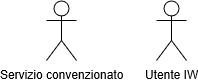
\includegraphics[width=0.5\columnwidth]{usecase/use-case-sp/attori.png} 
    \caption{Gerarchia utenti user case}
    \label{fig:ger-actors-sp} 
\end{figure}
\paragraph{Attori principali}
\begin{itemize}
    \item Servizio convenzionato: l’attore servizio convenzionato è quello che nell’analisi del dominio è stato definito come \textit{Real Service Provider} (RSP). Si tratta del fornitore reale del servizio.
    \item Utente IW: l’attore utente IW è una persona fisica che utilizza la nostra applicazione mobile al fine di operare l’accesso ad un servizio convenzionato in MonoKee.
\end{itemize}

\paragraph{Attori secondari}
Non sono presenti attori secondari.




\subsubsection{UC1: Azioni servizio convenzionato}
\begin{figure}[!htbp] 
    \centering 
    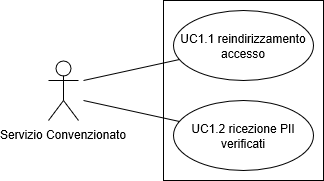
\includegraphics[width=0.7\columnwidth]{usecase/use-case-sp/UC1-Azioni-servizio-convenzionato.png} 
    \caption{Use Case - UC1: Azioni servizio convenzionato}
\end{figure}

\paragraph{Descrizione}  Il servizio convenzionato può reindirizzare verso al sistema una richiesta di accesso e ricevere i dati di accesso PII verificati.
\paragraph{Attore primario}  Servizio convenzionato
\paragraph{Attore secondario}  Nessuno
\paragraph{Precondizioni}  Il servizio convenzionato ha richiesto una richiesta di accesso e l’utente che l’ha effettuata a richiesto l’accesso tramite il nostro servizio.
\paragraph{Postcondizioni}  Il servizio ha eseguito le azioni che desiderava compiere in relazione alle sue possibilità
\paragraph{Scenario principale}  
    \begin{enumerate}
        \item UC1.1 Reindirizzamento accesso
        \item UC1.2 Ricezione PII verificati
    \end{enumerate}
\paragraph{Scenari alternativi}  Nessuno




\subsubsection{UC1.1: Reindirizzamento accesso}
\paragraph{Descrizione}  Un servizio convenzionato può inoltrare al sistema richieste di accesso
\paragraph{Attore primario}  Servizio convenzionato
\paragraph{Attore secondario}  Nessuno
\paragraph{Precondizioni}  Il servizio convenzionato ha ricevuto una richiesta di accesso
\paragraph{Postcondizioni}  Il sistema ha ricevuto la richiesta di accesso e procederà ad eseguirla
\paragraph{Scenario principale}  
Il servizio convenzionato inoltra la richiesta di accesso ed il sistema la immagazzina per prendersene carico
\paragraph{Scenari alternativi}  Nessuno



\subsubsection{UC1.2: Ricezione PII verificate}
\paragraph{Descrizione}  Il sistema deve, in risposta ad un inoltro di richiesta di accesso, inviare al servizio convenzionato l’esito della verifica e, in caso di successo, le PII in chiaro necessarie per effettuare l’oggetto
\paragraph{Attore primario}  Servizio convenzionato
\paragraph{Attore secondario}  Nessuno
\paragraph{Precondizioni}  Il servizio convenzionato ha precedentemente inoltrato una richiesta di accesso al sistema
\paragraph{Postcondizioni} Il sistema ha ricevuto l’esito della verificata ed in caso le PII necessarie per l’accesso in chiaro
\paragraph{Scenario principale}  
Il sistema riceve l’esito della verificata ed in caso le PII necessarie per l’accesso in chiaro
\paragraph{Scenari alternativi}  Nessuno



\subsubsection{UC2: Azioni utente IW}
\begin{figure}[!htbp] 
    \centering 
    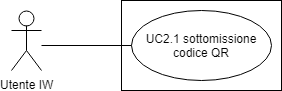
\includegraphics[width=0.7\columnwidth]{usecase/use-case-sp/UC2-Azioni-utente-SP.png} 
    \caption{Use Case - UC2: Azioni utente IW}
\end{figure}

\paragraph{Descrizione} L’utente IW può eseguire le operazioni per l’accesso
\paragraph{Attore primario}  Utente IW
\paragraph{Attore secondario}  \textit{MonoKee}
\paragraph{Precondizioni} Nessuna
\paragraph{Postcondizioni}  L’utente ha eseguito le azioni che desiderava compiere in relazione alla condizione.
\paragraph{Scenario principale}  
    \begin{enumerate}
        \item UC2.1 Sottomissione codice QR
    \end{enumerate}
\paragraph{Scenari alternativi}  Nessuno






\subsubsection{UC2.1: Sottomissione codice QR}
\paragraph{Descrizione}  L’utente IW può eseguire l’operazione di sottomissione di codice QR
\paragraph{Attore primario}  Utente IW
\paragraph{Attore secondario}  Nessuno
\paragraph{Precondizioni} Il servizio convenzionato ha inoltrato l’utente al nostro sistema di accesso e l’utente ha generato il codice QR dall’IW
\paragraph{Postcondizioni} Il sistema ha catturato il codice QR
\paragraph{Scenario principale}  
Il sistema accende la webcam del computer e cattura il codice QR che presenta l’utente.
\paragraph{Scenari alternativi}  Nessuno


\subsection{Diagramma delle attività}
Al fine di descrivere il corretto flusso che il componente deve utilizzare viene utilizzato un diagramma di attività. L’unica operazione che il componente dovrà gestire al fine di garantire gli scopi che si prefigge è la gestione di un inoltro d'accesso da parte di un RSP. 
\begin{figure}[!h]
    \centering
    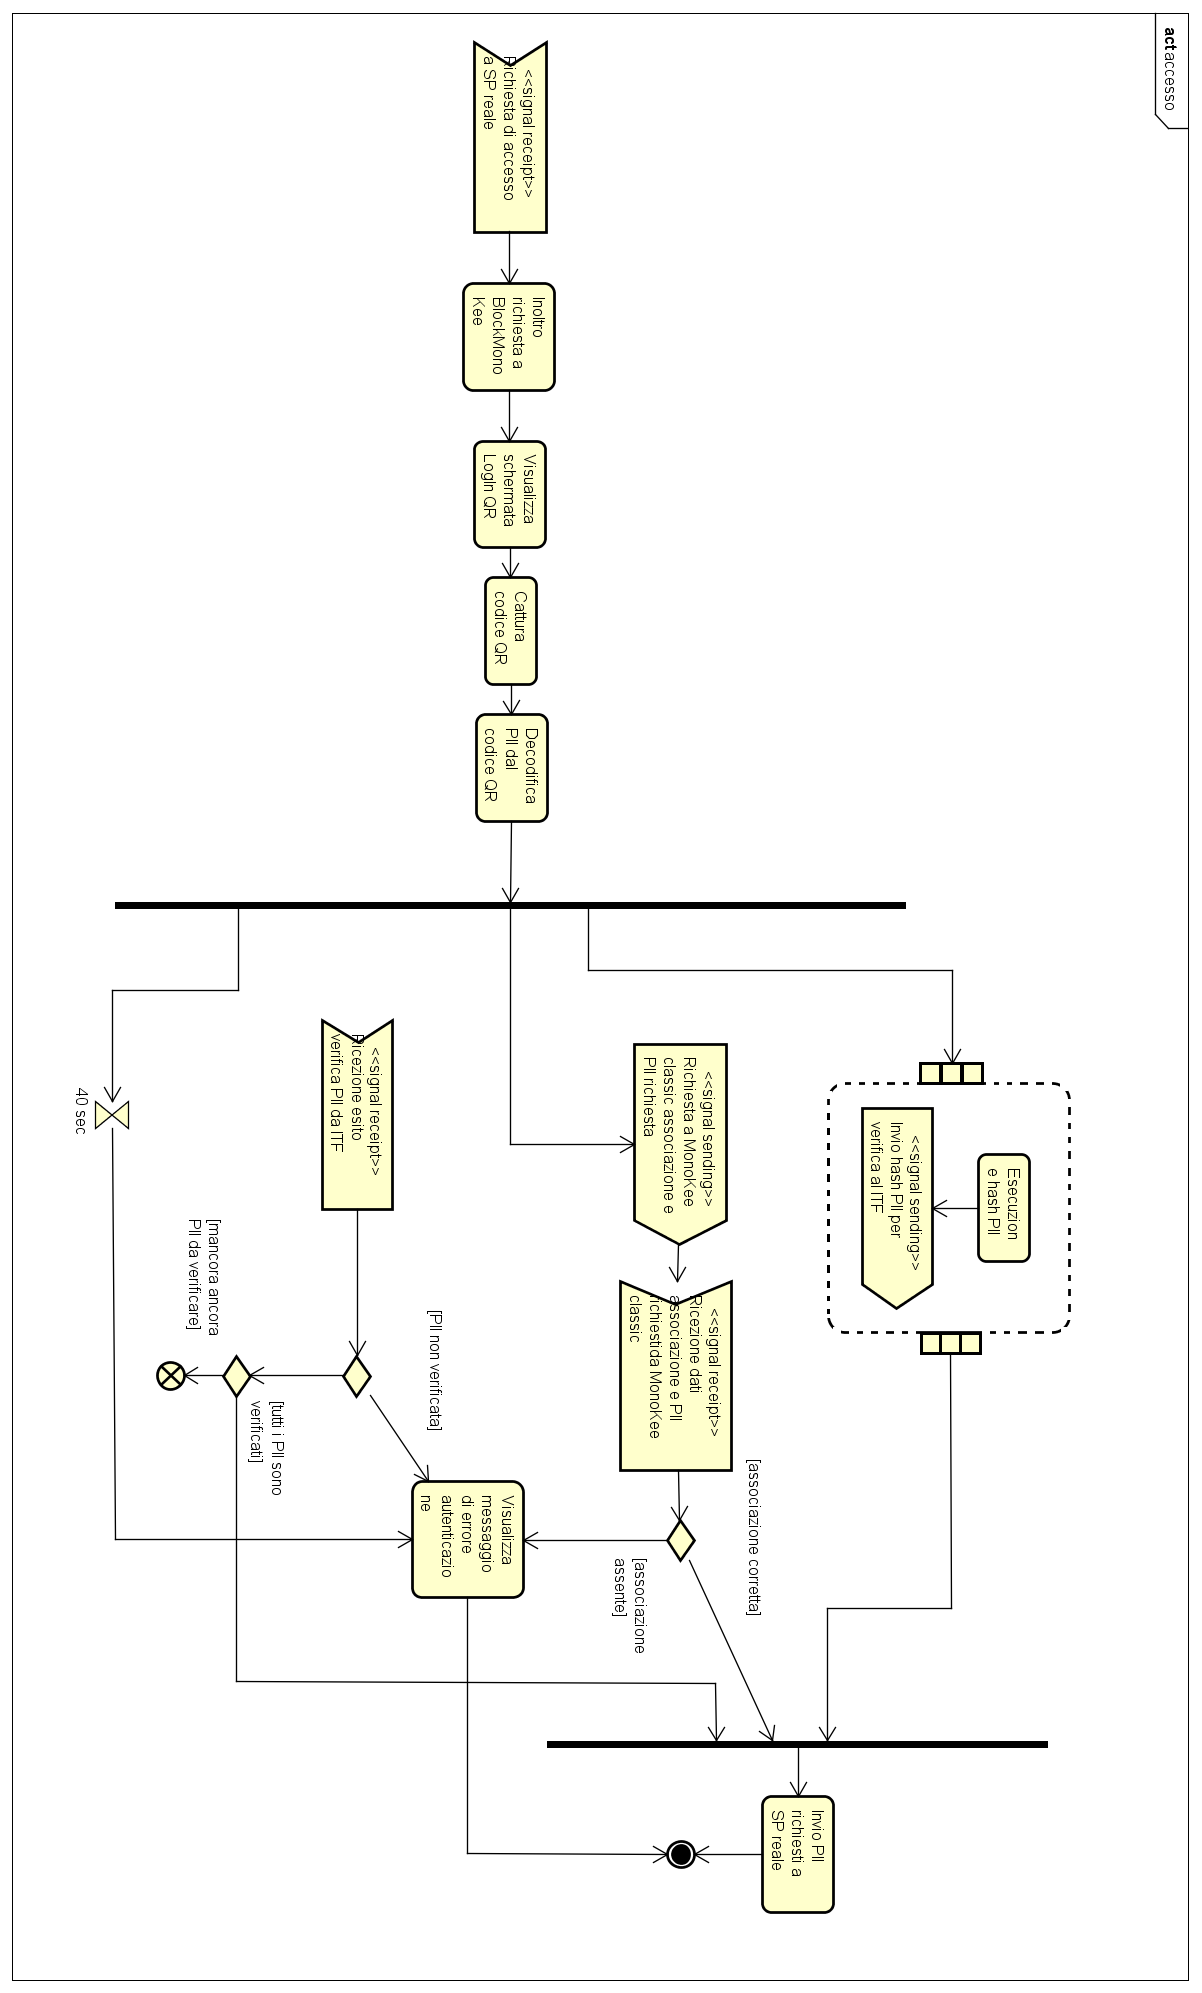
\includegraphics[width=1\columnwidth]{accesso.png} 
    \caption{Diagramma attività procedura di accesso}
    \label{fig:act-login} 
\end{figure}

Ora si procederà ad una breve descrizione del diagramma in figura ~\ref{fig:act-login}. 
Il flusso parte con l’arrivo di una richiesta di accesso da parte di un RSP, questo le seguenti operazioni in maniera sequenziale: 
\begin{itemize}
    \item inoltro della richiesta verso il nostro sistema SP;
    \item il sistema visualizza una schermata dove richiede la sottomissione del codice QR;
    \item cattura del codice QR;
    \item decodifica le PII in chiaro dal codice QR.
\end{itemize}


Poi il flusso si divide in tre operazioni differenti:
\begin{itemize}
    \item la prima con il compito di inviare una richiesta di verifica all’ITF per ogni PII decodificato dal codice QR;
    \item la seconda con il compito di interfacciarsi al sistema MonoKee per ottenere l’associazione tra account e servizio e la lista dei PII necessari;
    \item il terzo con il compito di aspettare gli esiti delle verifiche dall’ITF.
\end{itemize}
In caso l’associazione sia presente e corretta e tutte le PII necessarie sono verificate allora si procede con la comunicazione dei dati verso il reale fornitore del servizio.
In caso, o si riceva un esito negativo di una PII necessaria, o non tutte quelle necessarie siano state presentate tramite il codice QR, si procede alla comunicazione dell’errore di autentificazione ed alla conclusione del flusso.
In ogni caso se dopo 40 secondi dalla decodifica del codice QR il sistema non ha effettuato l’accesso viene visualizzato un messaggio di errore ed il flusso termina.

\subsection{Tracciamento dei requisiti}
\subsubsection{Fonti}
Per la deduzione dei requisiti utente e di sistema, che verranno presentati nelle sezioni a seguire, sono stati usati come fonti lo studio Gartner \footcite{farah:The-Dawn-of-Decentralized-Identity}, il capitolo \emph{Studio di fattibilità SP} e gli Use Case presentati nella sezione \emph{Casi d'uso}. La struttura e le convenzioni usate sono ispirate dal capitolo di \cite{som:swe}. In seguito vengono riportate le categorie che vengono usate per la catalogazione:
\begin{itemize}
    \item F: requisito funzionale;
    \item V: requisito di vincolo;
    \item Q: requisito di qualità.
\end{itemize}
    
Per l’attribuzione della priorità viene usata la tecnica \textit{MoSCoW}, quindi gli indici usati sono i seguenti:
\begin{itemize}
    \item M: must;
    \item S: should; 
    \item C: could; 
    \item W: will.
\end{itemize} 
    
Nelle tabelle \ref{tab:requisiti-funzionali-sp}, \ref{tab:requisiti-qualitativi-sp} e \ref{tab:requisiti-vincolo-sp} sono riassunti i requisiti e il loro tracciamento con gli \textit{use case} delineati in fase di analisi.

\newpage
\begin{center}
\begin{longtable}{|p{2cm}|p{9cm}|p{2cm}|}%
\caption{Tabella del tracciamento dei requisti funzionali}
\label{tab:requisiti-funzionali-sp}
\endfirsthead
\endhead
\hline
\textbf{Codice} & \textbf{Descrizione} & \textbf{Fonte}\\
\hline
R[F][M]0001     & Il sistema deve permettere ad un servizio convenzionato di inoltrare le richieste di accesso ricevute al nostro sistema & UC1, UC1.1, DA1 \\
\hline
R[F][M]0002     & Il sistema deve inviare l’esito della verifica al reale fornitore del servizio & UC1, UC1.2, DA1 \\
\hline
R[F][M]0003     & Il sistema deve inviare i PII in chiaro in caso di verifica positiva al reale fornitore del servizio & UC1, UC1.2, DA1 \\
\hline
R[F][M]0004     & Il sistema deve permettere ad un utente dell’IW di sottomettere un codice QR generato dall’applicazione IW. & UC2, UC2.1, DA1 \\
\hline
R[F][M]0005     & Il sistema deve visualizzare una schermata di accesso & DA1 \\
\hline
R[F][M]0006     & Il sistema deve catturare nella schermata di accesso il codice QR attraverso l’uso della webcam & DA1 \\
\hline
R[F][M]0007     & Il sistema deve essere in grado di decodificare le informazioni contenute in un codice QR & DA1 \\
\hline
R[F][M]0008     & Il sistema deve essere in grado di fare l’\textit{hash} di una PII & DA1 \\
\hline
R[F][M]0009     & Il sistema deve essere in grado di inviare una richiesta di verifica per un particolare PII  & DA1 \\
\hline
R[F][M]0010     & Il sistema deve essere in grado di eseguire l’operazione di hash e invio richiesta verifica per ogni PII presenta in un codice QR & DA1 \\
\hline
R[F][M]0011     & Il sistema deve inviare una richiesta dell’associazione utente-servizio a \textit{MonoKee} classico & DA1 \\
\hline
R[F][M]0012     & Il sistema deve essere in grado di ricevere le informazioni richiesta dell’associazione utente servizio da \textit{MonoKee} classico & DA1 \\
\hline
R[F][M]0013     & Il sistema deve visualizzare un messaggio di errore in caso cui l’associazione utente-servizio non sia presente per il servizio richiesto & DA1 \\
\hline
R[F][M]0014     & Il sistema deve essere in grado di ricevere l’esito della verifica di un singolo PII proveniente dall’ITF  & DA1 \\
\hline
R[F][M]0015     & Il sistema deve visualizzare un messaggio di errore in caso cui la verifica di una PII richiesta sia negativa & DA1 \\
\hline
R[F][M]0016     & Il sistema deve visualizzare un messaggio di errore in caso non tutte le verifiche delle PII necessarie tornino in 40 secondi. & DA1 \\
\hline
R[F][M]0017     & Il sistema deve in caso di presenza dell’associazione e del ritorno positivo di tutte le verifiche necessarie inviare i dati PII al SP reale & DA1 \\
\hline
\end{longtable}
\end{center}






\begin{center}
    \begin{longtable}{|p{2cm}|p{9cm}|p{2cm}|}%
    \caption{Tabella del tracciamento dei requisti di vincolo}
    \label{tab:requisiti-vincolo-sp}
    \endfirsthead
    \endhead
    \hline
    \textbf{Codice} & \textbf{Descrizione} & \textbf{Fonte}\\
    \hline
    R[V][M] 0018     & Il sistema deve offrire le proprie funzionalità come applicazione server centralizzata & SP Studio di fattibilità \\
    \hline
    B     & Il sistema è implementato tramite in linguaggi .NET & SP Studio di fattibilità \\
    \hline
    B     & Il progetto prevede almeno i seguenti quattro ambienti di sviluppo: \textit{Local}, \textit{Test}, \textit{Staging}, \textit{Production} & SP Studio di fattibilità \\
    \hline
    B     & Il prodotto è sviluppato utilizzando uno strumento di \textit{linting} & SP Studio di fattibilità \\
    \hline
    B     & Il sistema deve comunicare con la rete \textit{blockchain} tramite un \textit{client Ethereum}. & SP Studio di fattibilità \\
    \hline
    \end{longtable}
    \end{center}



    \begin{center}
        \begin{longtable}{|p{2cm}|p{9cm}|p{2cm}|}%
        \caption{Tabella del tracciamento dei requisiti qualitativi}
        \label{tab:requisiti-qualitativi-sp}
        \endfirsthead
        \endhead
        \hline
        \textbf{Codice} & \textbf{Descrizione} & \textbf{Fonte}\\
        \hline
        R[Q][S] 0023    & Il progetto prevede un ragionevole set di test di unità e di test di integrazione & - \\
        \hline
        R[Q][S] 0024   & I test possono essere eseguiti localmente o come parte di integrazione continua & - \\
        \hline
        R[Q][S] 0025    & Il sistema solo alla fine sarà testato nel server di prova & - \\
        \hline
        R[Q][S] 0026    & Il codice sorgente del prodotto e la documentazione necessaria per l’utilizzo sono versionati in repository pubblici usando GitHub, BitBucket o GitLab & - \\
        \hline
        R[Q][C] 0027    & Lo sviluppo si eseguirà utilizzano un approccio incrementale  & SP Studio di fattibilità \\
        \hline
        R[Q][C] 0028    & Il sistema potrebbe essere testato con l’ITF migrato nella rete di prova Ropsten  & ITF Studio tecnologico \\
        \hline
        \end{longtable}
        \end{center}%




        \begin{center}
            \begin{longtable}{|p{3cm}|p{3cm}|}%
            \caption{Tabella del tracciamento dei requisiti con le fonti}
            \label{tab:requisiti-fonte-sp}
            \endfirsthead
            \endhead
            \hline
            \textbf{Codice}  & \textbf{Fonte}\\
            \hline
            R[F][M]0001    & UC1, UC1.1, DA1  \\
            \hline
            R[F][M]0002    & UC1, UC1.1, DA1  \\
            \hline
            R[F][M]0003    & UC1, UC1.1, DA1  \\
            \hline
            R[F][M]0004    & UC2, UC2.1, DA1  \\
            \hline
            R[F][M]0005    & DA1  \\
            \hline
            R[F][M]0006    & DA1  \\
            \hline
            R[F][M]0007    & DA1  \\
            \hline
            R[F][M]0008    & DA1  \\
            \hline
            R[F][M]0009    & DA1  \\
            \hline
            R[F][M]0010    & DA1  \\
            \hline
            R[F][M]0011    & DA1  \\
            \hline
            R[F][M]0012    & DA1  \\
            \hline
            R[F][M]0013    & DA1  \\
            \hline
            R[F][M]0014    & DA1  \\
            \hline
            R[F][M]0015    & DA1  \\
            \hline
            R[F][M]0016    & DA1  \\
            \hline
            R[F][M]0017    & DA1  \\
            \hline
            R[V][M] 0018    & SP Studio di fattibilità  \\
            \hline
            R[V][M] 0019    & SP Studio di fattibilità  \\
            \hline
            R[V][M] 0020    & SP Studio di fattibilità  \\
            \hline
            R[V][M] 0021    & SP Studio di fattibilità  \\
            \hline
            R[V][C] 0022    & SP Studio di fattibilità  \\
            \hline
            R[Q][S] 0023    & -  \\
            \hline
            R[Q][S] 0024    & -  \\
            \hline
            R[Q][S] 0025    & -  \\
            \hline
            R[Q][S] 0026    & -  \\
            \hline
            R[Q][C] 0027    & SP Studio di fattibilità  \\
            \hline
            R[Q][C] 0028    & ITF Studio tecnologico  \\
            \hline
            \end{longtable}
            \end{center}%

    \begin{center}
        \begin{longtable}{|p{3cm}|p{3cm}|}%
        \caption{Tabella del tracciamento dei fonte con requisiti}
        \label{tab:fonti-req-sp}
        \endfirsthead
        \endhead
        \hline
        \textbf{Fonte}  & \textbf{Requisiti}\\
        \hline
        UC1    & R[F][M]0001
        R[F][M]0002
        R[F][M]0003  \\
        \hline
        UC2    & R[F][M]0004  \\
        \hline
        UC1.1    & R[F][M]0001  \\
        \hline
        UC1.2    & 
        R[F][M]0002
        R[F][M]0003  \\
        \hline
        UC2.1    & R[F][M]0004  \\
        \hline
        DA1    & R[F][M]0001
        R[F][M]0002
        R[F][M]0003
        R[F][M]0004
        R[F][M]0005
        R[F][M]0006
        R[F][M]0007
        R[F][M]0008
        R[F][M]0009
        R[F][M]0010
        R[F][M]0011
        R[F][M]0012
        R[F][M]0013
        R[F][M]0014
        R[F][M]0015
        R[F][M]0016
        R[F][M]0017  \\
        \hline
        SP Studio di fattibilità    & 
        R[V][M]0018
        R[V][M]0019
        R[V][M]0020
        R[V][M]0021
        R[V][M]0022
        R[Q][C]0027  \\
        \hline
        -    & 
        R[Q][S]0023
        R[Q][S]0024
        R[Q][S]0025
        R[Q][S]0026  \\
        \hline
        ITF Studio tecnologico    & R[Q][C]0028  \\
        \hline

        \end{longtable}
        \end{center}%

\section{Riepilogo requisiti}

\subsection{Riepilogo requisiti IW}
In tabella ~\ref{tab:riepilogo-req-iw} vengono riportati la quantità dei requisiti individuati per l'IW suddivisi
per tipo e per priorità.
\begin{center}
    \begin{longtable}{|p{2cm}|p{2cm}|p{2cm}|p{2cm}|p{2cm}|}
    \caption{Riepilogo requisiti IW}
    \label{tab:riepilogo-req-iw}
    \endfirsthead
    \endhead
    \hline
    \textbf{Categoria}  & \textbf{Must} & \textbf{Should} & \textbf{Could} & \textbf{Will}\\
    \hline
    \textbf{Funzionale} & 21 & 1 & 4 & 0 \\
    \hline
    \textbf{Di vincolo} & 5 & 0 & 0 & 0 \\
    \hline
    \textbf{Di qualità} & 0 & 4 & 1 & 0 \\
    \hline
    \end{longtable}
    \end{center}%
\subsection{Riepilogo requisiti SP}
In tabella ~\ref{tab:riepilogo-req-sp} vengono riportati la quantità dei requisiti individuati per l'SP suddivisi
per tipo e per priorità.
\begin{center}
    \begin{longtable}{|p{2cm}|p{2cm}|p{2cm}|p{2cm}|p{2cm}|}
    \caption{Riepilogo requisiti SP}
    \label{tab:riepilogo-req-sp}
    \endfirsthead
    \endhead
    \hline
    \textbf{Categoria}  & \textbf{Must} & \textbf{Should} & \textbf{Could} & \textbf{Will}\\
    \hline
    \textbf{Funzionale} & 17 & 0 & 0 & 0 \\
    \hline
    \textbf{Di vincolo} & 4 & 0 & 1 & 0 \\
    \hline
    \textbf{Di qualità} & 0 & 4 & 2 & 0 \\
    \hline
    \end{longtable}
    \end{center}%